If the parameters are in an wide acceptable range that we will define later, all the execution are alike, because the limiting factor are the shapes of the templates. This prevents the algorithm to surpass a certain level of quality, and makes many different parameters combinations to be equivalent in terms of result quality.\\
We describe here the behavior of the errors during one of these typical equivalent runs (parameters : $\sigma=5$, $\lambda=11$, $U^{global}=5\% $, $\frac{U^{add}}{\widetilde{F}}=5\% $, $U^{mul}=75 \% $).\\
\\
\emph{$E_{proj}$}: By construction, $E_{proj}$ is always very close to zero at the end of the execution (the algorithm come closer and closer to the feasible space).\\
Fig. \ref{fig:eprojexample}. illustrates this behavior on a typical example.\\ 
\begin{figure}[!h]
	\caption{Evolution of $E_{proj}$ during a typical execution}
	\label{fig:eprojexample}
	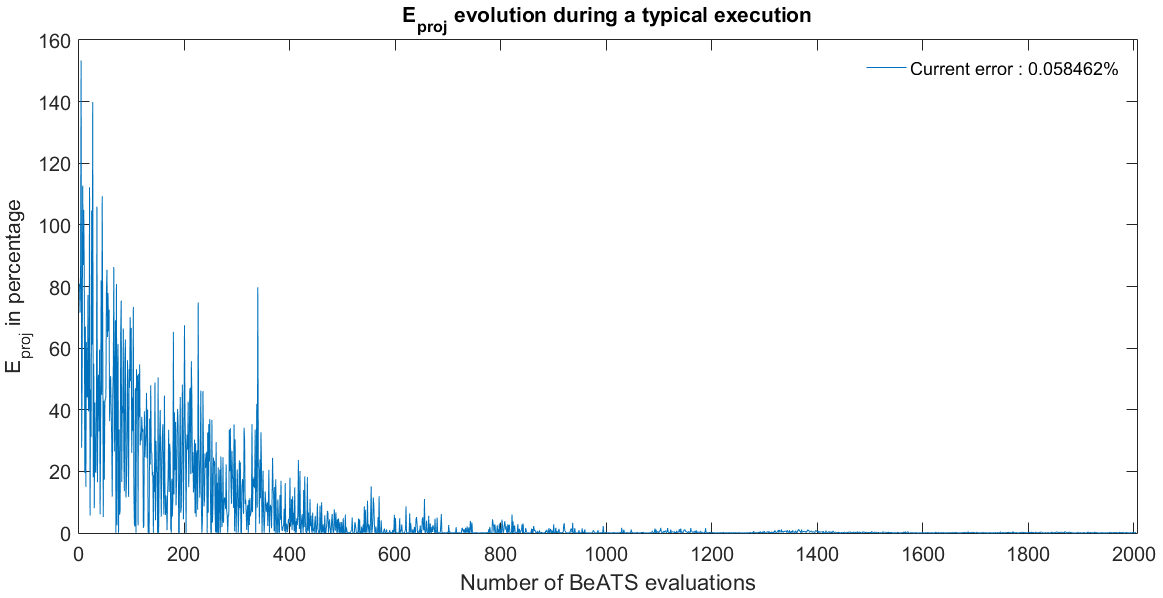
\includegraphics[width=7in]{figures/results_figures/eprojexample.png}
\end{figure}	
\newpage 
\emph{$E_{VMT}$}: By imputation, as explained in \ref{subsubsec:tvm} and \ref{subsec:implementation}, $E_{VMT}$ is always below $5\%$, often around $1-2\%$ on each iteration of the algorithm.\\
Fig. \ref{fig:vmtexample} reflects the history of $VMT$ during a typical run.\\
\begin{figure}[!h]
	\caption{Evolution of $E_{VMT}$ during a typical execution}
	\label{fig:vmtexample}
	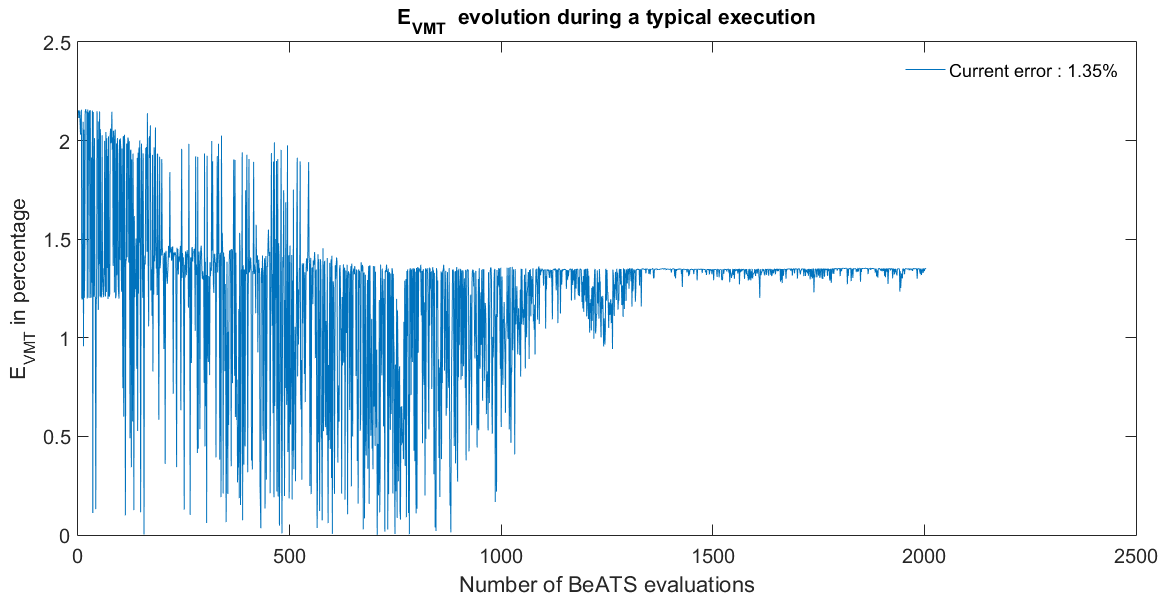
\includegraphics[width=7in]{figures/results_figures/VMTexample.png}
\end{figure}	
\newpage
\emph{$E_{VHT}$}: VHT is quite correlated with the congestion : on the typical executions that lead to an acceptable congestion, $E_{VHT}^{*}$ is around $U^{global}=5\%$. However, particularly when the knobs are constrained too much,  $E_{VHT}^{*}$ ends up around $20\%$.
Fig. \ref{fig:vhtexample} reflects the history of $E_{VHT}$ with its typical -good- behavior.
\begin{figure}[!h]
	\caption{Evolution of $VHT$ during a typical execution}
	\label{fig:vhtexample}
	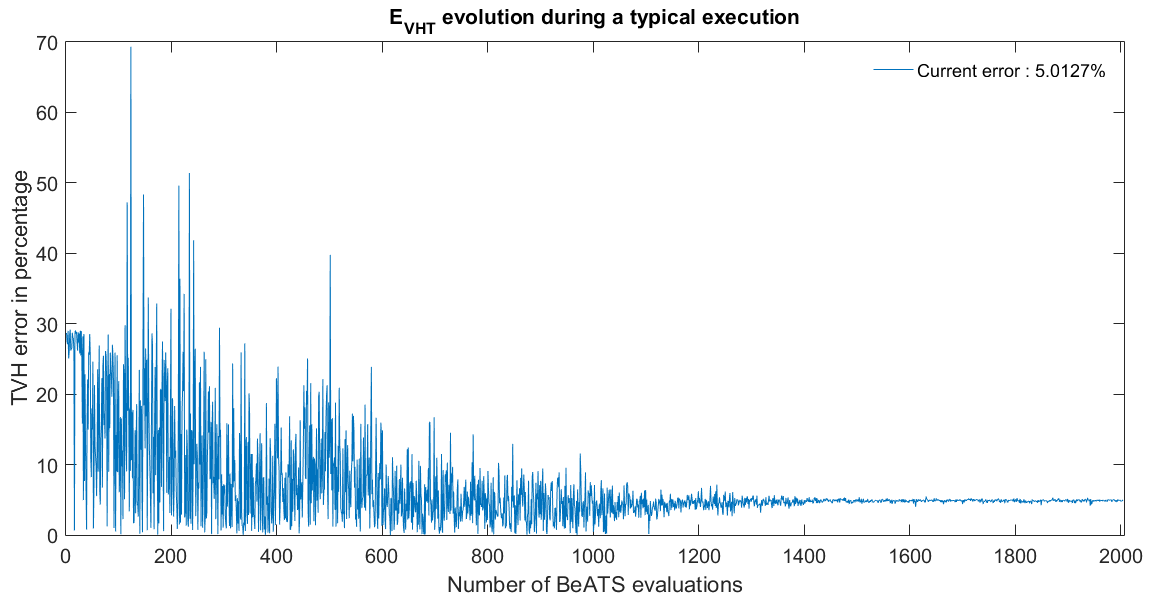
\includegraphics[width=7in]{figures/results_figures/VHTexample.png}
\end{figure}\\
\emph{$E_{CP}$}: $E_{CP}$ behaves like $E_{VHT}$. The congestion shape obtained for the typical run (best we got) is displayed in Fig. \ref{fig:typicalcpexample}. This shape is obtained for all the executions that have acceptable parameters. We can see the two congestion patterns induced by the templates : the smaller one in the morning is correlated with the bigger one in the afternoon and impossible to suppress.
\begin{figure}[!h]
	\caption{Typical congestion pattern fitting result}
	\label{fig:typicalcpexample}
	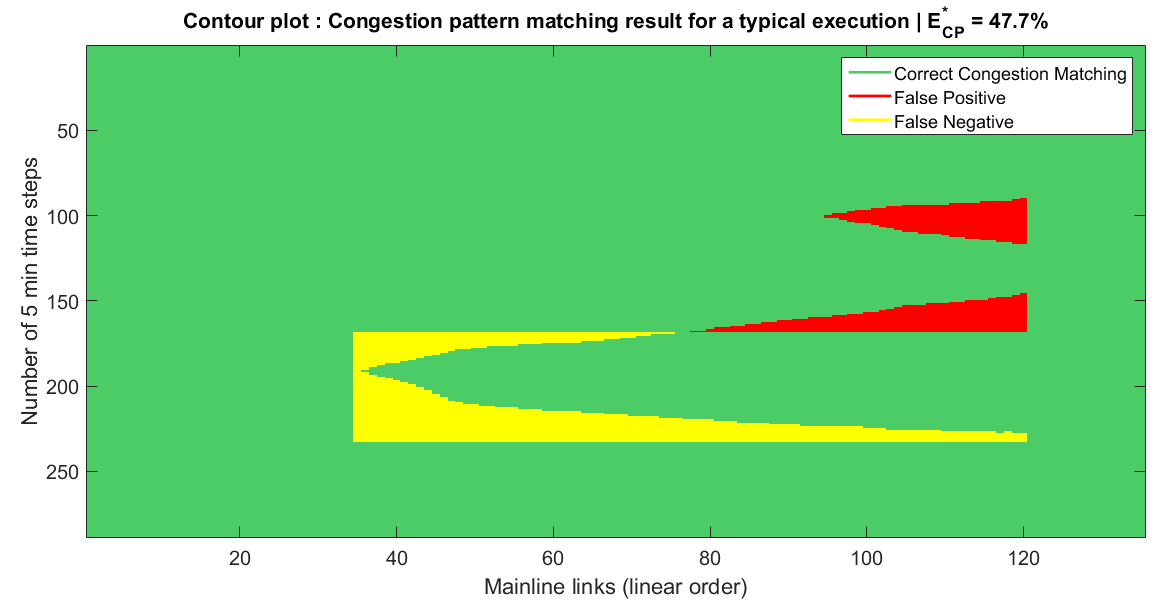
\includegraphics[width=7in]{figures/results_figures/typicalcpexample.png}
\end{figure}	
\newpage
Fig. \ref{fig:contributionsexample} displays the evolution of the contributions $\phi_{CP}$, $\phi_{VMT}$, $\phi_{VHT}$ and $\phi_{proj}$ of every parameter and their sum, the global error $\Phi$.\\
\begin{figure}[!h]
	\caption{$\Phi$ and contributions evolution during a typical execution}
	\label{fig:contributionsexample}
	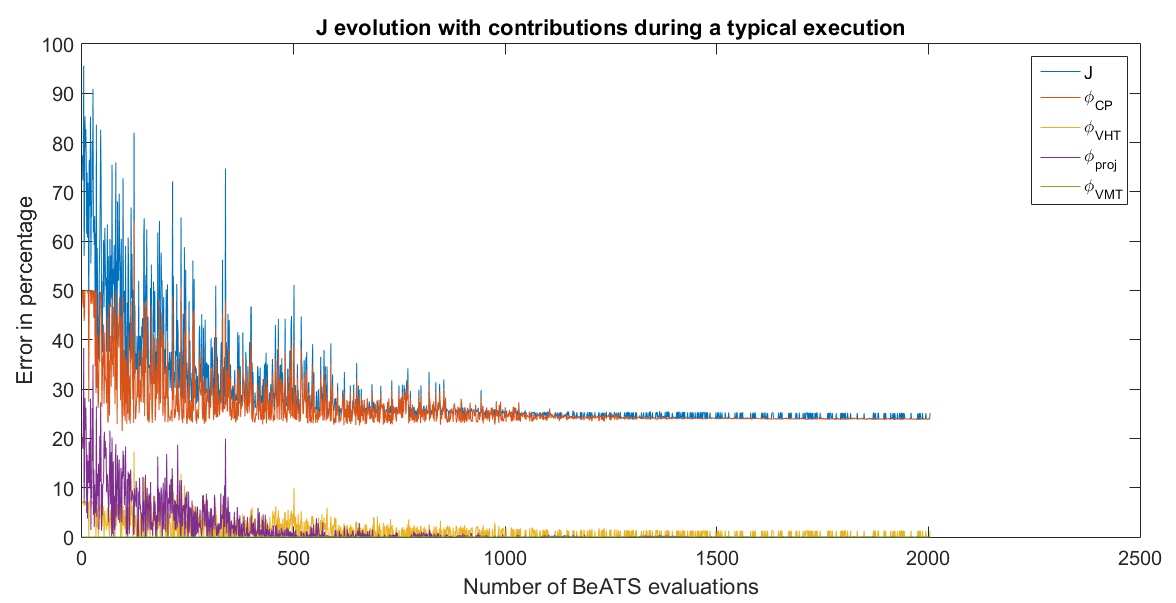
\includegraphics[width=7in]{figures/results_figures/contributionsexample.png}
\end{figure}	
\\
Fig. \ref{fig:typicalknobs} shows the evolution of the knobs during the execution of CMA-ES (we will call it "knobs history").
\begin{figure}[!h]
	\caption{[0-10] knobs history during a typical CMA-ES execution.}
	\label{fig:typicalknobs}
	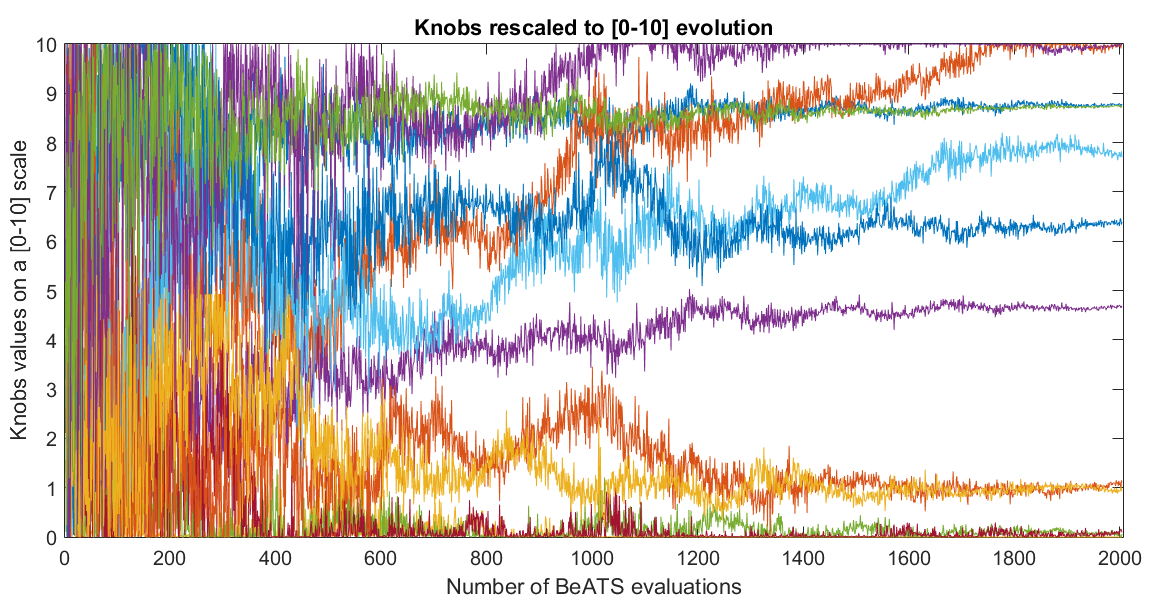
\includegraphics[width=7in]{figures/results_figures/typicalknobs.png}
\end{figure}
\newpage
Finally, the following figure \ref{fig:cmaesexample} displays the evolution of the standard deviations associated  in CMA-ES to each knob.
\begin{figure}[!h]
	\caption{CMA-ES parameters evolution during a typical execution}
	\label{fig:cmaesexample}
	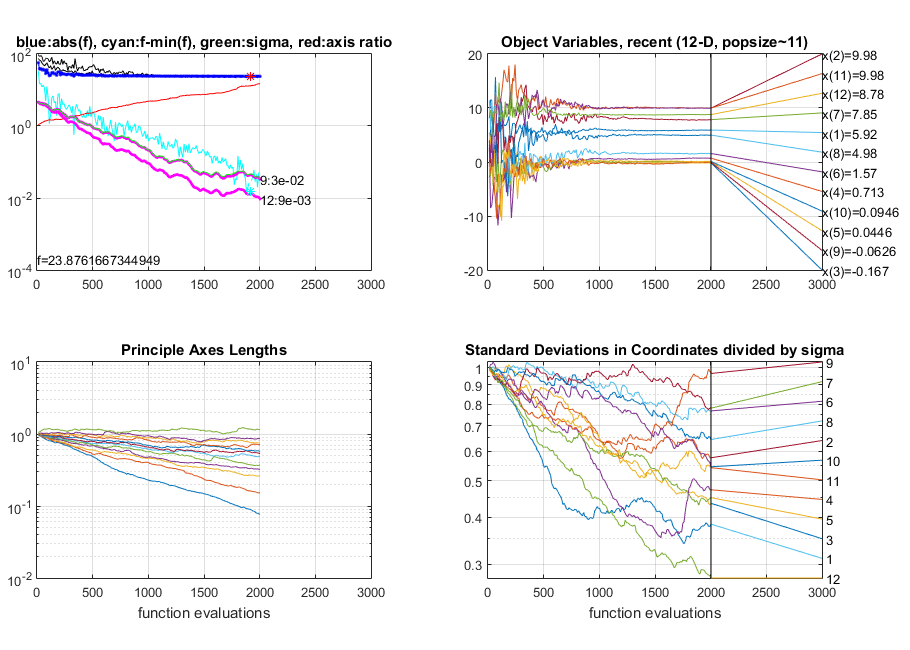
\includegraphics[width=7in]{figures/results_figures/cmaesexample.png}
\end{figure}	


